\documentclass[10pt]{article}
\usepackage[utf8]{inputenc}
\usepackage[spanish]{babel}
\usepackage{amsmath}
\usepackage{amsfonts}
\usepackage{amssymb}
\usepackage{graphics}
\usepackage{graphicx}
\usepackage[left=2cm,right=2cm,top=2cm,bottom=2cm]{geometry}
\usepackage{imakeidx}
\makeindex[columns=3, title=Alphabetical Index, intoc]
\usepackage{listings}
\usepackage{xcolor}
\usepackage{multicol}
\usepackage{changepage}
\usepackage{float}
\usepackage{cite}
\usepackage{url}
\usepackage{hyperref}
\usepackage{pdflscape}
\usepackage[document]{ragged2e}
\hypersetup{
    colorlinks=true,
    linkcolor=blue,
    filecolor=magenta,
    urlcolor=blue,
}

\definecolor{codegreen}{rgb}{0,0.6,0}
\definecolor{codegray}{rgb}{0.5,0.5,0.5}
\definecolor{codepurple}{rgb}{0.58,0,0.82}
\definecolor{backcolour}{rgb}{0.95,0.95,0.92}

\lstdefinestyle{mystyle}{
    backgroundcolor=\color{backcolour},
    commentstyle=\color{codegreen},
    keywordstyle=\color{magenta},
    numberstyle=\tiny\color{codegray},
    stringstyle=\color{codepurple},
    basicstyle=\ttfamily\footnotesize,
    breakatwhitespace=false,
    breaklines=true,
    captionpos=b,
    keepspaces=true,
    numbers=left,
    numbersep=5pt,
    showspaces=false,
    showstringspaces=false,
    showtabs=false,
    tabsize=3
}
\def\fillandplacepagenumber{%
 \par\pagestyle{empty}%
 \vbox to 0pt{\vss}\vfill
 \vbox to 0pt{\baselineskip0pt
   \hbox to\linewidth{\hss}%
   \baselineskip\footskip
   \hbox to\linewidth{%
     \hfil\thepage\hfil}\vss}}
\lstset{style=mystyle}

\title{Centro de Investigación en Cómputo\\Instituto Politécnico Nacional\\Metaheurísticas\\Actividad No. 17\\Solución de problemas mediante Algoritmos Genéticos Estacionarios\\Curso impartido por: Dra Yenny Villuendas Rey}

\author{Adrian González Pardo}

\date{\today}

\newcommand\tab[1][1cm]{\hspace*{#1}}

\begin{document}
\maketitle
\section{Ventajas y Desventajas de GA}
\begin{center}
  \begin{tabular}{|p{6cm}|p{6cm}|}
    \hline
    Ventajas & Desventajas \\
    \hline
    Permite realizar multiples busqueda de soluciones a los problemas & Puede que el metodo de mutación o cruza seleccionado puede que no ayude a encontrar una buena solución\\
    \hline
    Esta bioinspirado en la genética y en la selección natural (Darwinismo) & Puede que el que en la aplicación en alguna etapa del GA ya no avance \\
    \hline
    Es una heurística poblacional & Puede que genere bastante uso de recursos en memoria y procesamiento \\
    \hline
    Es posible el trabajar soluciones de formas paralelizables o distribuidas&Puede ser dificil de implementar\\
    \hline
  \end{tabular}
\end{center}
\section{Genotipo vs Fenotipo}
\textbf{Genotipo:} es una representación en cadenas de bits en la cual generalmente es trabajada para generar un nuevo individuo en el algoritmo.
\\
\textbf{Fenotipo:} es la representación que tiene la cadena de bits en el ambito del problema, es decir, la cadena de bits puede representar números reales $\mathbb{R}$, números enteros $\mathbb{Z}$, valores binarios $\{0,1\}$, indices de la solución a algún problema.

\section{Operadores}
\subsection{Mutación}
\subsubsection{Aleatoria para fenotipo real}
Para este tipo de mutación es necesario conocer la dimensión del arreglo, de modo en que para la mutación de este tipo podemos hacer dos metodos distintos hacer la modificación mediante una selección aleatoria en cualquier $x_{i}$ con valores aleatorios que van de $[min,max]$ y la otra que itera sobre cada $x_{i}$ bajo una función de probabilidad cuyo valor es pequeño y si se genera un valor aleatorio cuyo valor compite en la función de probabilidad y este es menor se generara el valor aleatorio en el intervalo del metodo anterior.
\subsubsection{Aleatoria para fenotipo binario}
Para esta mutación se hara uso de un valor de probabilidad pequeño de modo en que se debe obtener un valor pequeño de tal modo que este significara que hay una modificación sobre cada bit particular $b_{i}={0,1}$ de tal forma en que se puede realizar esto con cada indice $b_{i}$ o se puede iterar sobre todos y cada uno de ellos
\subsubsection{Aleatorio para fenotipo de orden}
Para este tipo de mutación al igual que los anteriores podemos apoyarnos del uso del valor de probabilidad para mutar sobre dos valores $p_{i}$ que intercambia lugar con $p_{j}$ de tal modo en que mediante esta permutación podremos generar una nueva solución, por otro lado se puede realizar esta permutación una sola ocasión o realizarla como si se iterara sobre cada elemento de la solución es decir $N$ veces
\subsection{Cruzamiento}
\subsubsection{Dos puntos de corte}
Es una forma de intercambiar información entre dos padres. Esta forma de cruce se selecciona dos puntos aleatorios de corte de forma que se los cortes van de $[1,a],[a,b],[b,N-1]$, quedando un ejemplo de la siguiente forma:
\begin{center}
  \begin{tabular}{|c|c|c|c|c|c|c|c|}
    \hline
    \color{green}0&\color{green}0&\color{green}0&\color{green}1&\color{blue}1&\color{blue}0&\color{green}1&\color{green}1\\
    \hline
    \color{red}1&\color{red}0&\color{red}1&\color{red}0&\color{yellow}0&\color{yellow}1&\color{red}1&\color{red}0\\
    \hline
  \end{tabular}
  \textbf{Pasan a:}
  \begin{tabular}{|c|c|c|c|c|c|c|c|}
    \hline
    \color{green}0&\color{green}0&\color{green}0&\color{green}1&\color{yellow}0&\color{yellow}1&\color{green}1&\color{green}1\\
    \hline
    \color{red}1&\color{red}0&\color{red}1&\color{red}0&\color{blue}1&\color{blue}0&\color{red}1&\color{red}0\\
    \hline
  \end{tabular}
\end{center}

\subsubsection{Uniforme}
Este tipo de cruzamiento se realiza bajo un vector con valores de probabilidad, destacando que cada elemento del arreglo tiene una probabilidad de cruza del $0.5$ por lo que generaran valores aleatorios en el vector de tal manera que si $v_{i}\geq 0.5$ este indice realiza la cruza de datos de ese indice.\\Un ejemplo de ello seria el siguiente:
\textbf{Se genera un vector con los siguientes datos}
\begin{center}
  \begin{tabular}{|c|c|c|c|c|c|c|c|}
    \hline
    0.55 & 0.03 & 0.67 & 0.77 & 0.30 & 0.25 & 0.99 & 0.78 \\
    \hline
  \end{tabular}
  \\\vspace{0.25cm}
  \textbf{Teniendo los siguientes padres:}\\
  \begin{tabular}{|c|c|c|c|c|c|c|c|}
    \hline
    \color{blue}0&\color{blue}0&\color{blue}0&\color{blue}1&\color{blue}1&\color{blue}0&\color{blue}1&\color{blue}1\\
    \hline
    \color{red}1&\color{red}0&\color{red}1&\color{red}0&\color{red}0&\color{red}1&\color{red}1&\color{red}0\\
    \hline
  \end{tabular}
  \textbf{Entonces:}
  \begin{tabular}{|c|c|c|c|c|c|c|c|}
    \hline
    \color{red}1 & \color{blue}0 & \color{red}1 & \color{red}0  & \color{blue}1 & \color{blue}0 & \color{red}1&\color{red}0\\
    \hline
    \color{blue}0 & \color{red}0 & \color{blue}0 & \color{blue}1  & \color{red}0 & \color{red}1 & \color{blue}1&\color{blue}1\\
    \hline
  \end{tabular}
\end{center}
\subsubsection{Aritmético}
Para este tipo de algoritmo es necesario pensar en que nuestros dos vectores padres son valores reales los cuales van a ser cruzados a traves de un valor aleatorio $\alpha\in[0,1]$ de modo que actuaran como valores escalares para nuestros vectores, de tal forma que existe un segundo valor $\beta=1-\alpha$ formando la siguiente ecuación para realizar la cruza:\\\vspace{0.25cm}
Sean los vectores \\
\[\displaystyle X^{1}={x_0^{1},x_1^{1},\cdots,x_N^{1}}\] \[\displaystyle X^{2}={x_0^{2},x_1^{2},\cdots,x_N^{2}}\]
\[y=\alpha x^{1}+\beta x^{2}\]
\subsection{Selección}
\subsubsection{Torneo}
Este modelo se trata de ir realizando un $k$ número de arreglos permutados de forma aleatoria de tamaño $N$ que es el tamaño dimensional de la respuesta de tal modo en que se busca seleccionar el valor indice de aquellos datos que esten mejor evaluados en el torneo, gráficamente el torneo se ve de la siguiente manera:\\
\(\displaystyle k=2\), entonces \(\displaystyle [0.5,1,4,0.1]\), la generación aleatoria, generaria lo siguiente por ejempo:\\
\begin{center}
  \begin{tabular}{|c|c|c|c|}
    \hline
    2&1&4&3\\
    \hline
    4&2&3&1\\
    \hline
  \end{tabular}\\
  \textit{Se accedera a los valores de cada subindice del arreglo en su valor y se evaluara el menor valor vía indices es decir de arriba hacia abajo para seleccionar al mejor.}\\
  \begin{tabular}{|c|c|c|c|}
    \hline
    4&1&4&1\\
    \hline
  \end{tabular}
\end{center}

\subsubsection{Proporcional}
Para este tipo de selección se usa la función
\[p_{i}=\cfrac{f_{i}}{\sum_{j=1}^{N}f_{j}}\]
Donde:\\
\(\displaystyle p_i\) es la probabilidad de ser seleccionado \(\displaystyle p_{i}\)\\\vspace{0.25cm}
\(\displaystyle f_{i}\) es la función de fitness para ese valor de \(\displaystyle i\)\\\vspace{0.25cm}
Por tanto al obtener esto tendremos un pequeño sesgo probabilistico a la hora de seleccionar un área por tanto definiremos al error selectivo como:
\[n_{i}=p_i\;\times\;N\;=\;\left\lfloor\;N\;\times\;\cfrac{f_{i}}{\sum_{j=1}^{N}f_{j}}\right\rfloor\]
En esta ecuación nos podremos percatar de que redondeamos el error a un valor entero, lo que significa que cada individuo podría perderse cualquiera que sea su valor relativo de aptitud.

\subsubsection{Por Emparejamiento Variado Inverso (NAM)}
Un padre se escoge aleatoriamente, para el otro selecciona Nnam padres y escoge el más lejano al primer (\(\displaystyle Nnam=3,5,\cdots\)). Está orientado a generar diversidad.
\section{Impacto en convergencia a la solución con GA}
Como bien sabemos la existencia de un algoritmo bioinspirado en la selección natural y el la biología en si misma nos hace pensar que en cuestion de generación de soluciones ya sean aleatorias en cada nueva iteración o con alguna conservación en sus estados es de suma importancia ya que de este modo podemos explorar ya sea de forma continua o paralela el espacio de soluciones de modo en que se puede converger en la solución al problema de una forma más rápida y sencilla, por lo que a mayor tamaño de población podría significar mayor procesamiento pero si se implementa alguna técnica de paralelización pueda que en tiempo sea casi aproximado a las soluciones de los otros algoritmos heurísticos como lo son Random-Mutation Hill-Climbing (RMHC) o Simulated Annelling (SA).


\section{Estructuras de datos necesarias para la implementación en problemas}
\subsection{Knapsack}
Modelación Matemática\\
Sean dos funciones
\[f(x)=\sum_{i=1}^{N}x^{'}_{i}h(x_{i})\]
\[g(x)=\sum_{i=1}^{N}x^{'}_{i}p(x_{i})\;\leq\;peso\_m\acute{a}ximo\]
Donde:\\
\(\displaystyle X\;es\;un\;vector\;de\;la\;forma\;X=[x_{1},x_{2},\cdots,x_{N}]\)\\\vspace{0.25cm}
\(\displaystyle X^{'}\;es\;un\;vector\;el\;cual\;es\;parecido\;a\;X\;pero\;sus\;valores\;son\;binarios\;x_{i}^{'}\in\{0,1\}\)\\\vspace{0.25cm}
\(\displaystyle h(x_{i})\;es\;una\;funci\acute{o}n\;la\;cual\;devuelve\;el\;beneficio\;total\;de\;los\;objetos\;x_{i}\;en\;la\;mochila\)\\\vspace{0.25cm}
\(\displaystyle p(x_{i})\;es\;una\;funci\acute{o}n\;la\;cual\;devuelve\;el\;peso\;total\;de\;los\;objetos\;x_{i}\;en\;la\;mochila\)\\\vspace{0.25cm}
De modo que para los operadores GA en este problema el genotipo puede ser la cadena de bits de modo que el fenotipo que representa de la cadena es la representación de un valor binario de si el objeto es incluido o no es incluido en la solución.\\
Finalmente la estructura de datos para esta solución es un arreglo binario el cual contendra un valor $0$ o $1$ de tal forma en que se pueda veter cada arreglo a la selección y torneo de GA, por tanto así podria calcularle los valores de su función de maximización de beneficio y de tratar de minimizar o no sobrepasar el peso máximo de la mochila
\subsection{Travel Salesman Problem (TSP)}
Modelación Matemática\\
Sea la función
\[f(x)=\sum_{i=1}^{N}x_{i} \cdot g\left(y_{x_{i},i}\right)\]
Donde:\\
\(\displaystyle Y\;es\;una\;matriz\;de\;NxN\;la\;cual\;trabajara\;para\;obtener\;el\;costo\;con\;la\;funci\acute{o}n\;g(x)\)\\\vspace{0.25cm}
\(\displaystyle X\;es\;un\;vector\;de\;dimensi\acute{o}n\;N\;el\;cual\;contiene\;el\;\acute{i}ndice\;del\;v\acute{e}rtice\;al\;cual\;pasa\;de\;i\;a\;j\)\\\vspace{0.25cm}
\(\displaystyle g(y_{x_{i},i})\;es\;una\;funci\acute{o}n\;la\;cual\;devuelve\;el\;costo\;de\;ir\;de\;i\;hacia\;el\;contenido\;de\;x_{i}\)\\\vspace{0.25cm}
De modo en que nuestro GA puede ser implementado con un fenotipo entero el cual representa la ciudad n hacia que vértice se conecta posteriormente.\\\vspace{0.25cm}
\textit{Ejemplo de arreglo $X$: }\(\displaystyle x=[2,3,1,0]\) de modo que sabemos que nuestro grafo tiene $4$ aristas y pensando en que todos están conectados partiremos de la siguiente manera $(0\rightarrow 2),\;(2\rightarrow 1),\;(1\rightarrow 3),\;(3\rightarrow 0)$ de tal forma que el formato en como realiza el movimiento de un vértice a otro es $(i\rightarrow j)$ siendo el valor de $j$ el que sera evaluado en la matriz $Y$ para obtener su costo.\\
Finalmente para este es tan sencillo como la realización de un arreglo de orden que contenga los valores de cada nodo o ciudad de la solución para así realizar el cálculo de su costo y así sobre cada solución.
\subsection{Función de Minimización en D dimensiones}
Modelación Matemática\\
Sea la función
\[f(x)=\sum_{i=1}^{D}x_{i}^{2}\]
Donde:\\
\(\displaystyle x_{i}\in\mathbb{R}\)\\\vspace{0.25cm}Descrito en los intervalos \(\displaystyle x_{i}\in[-10,10]\)\\\vspace{0.25cm}
Donde sabemos que los puntos mínimos de cada $x_{i}$ los encontramos cuando el valor asignado a el es $x_{i}=0$ por lo tanto el ir variando los valores para que el programa se acerque hacia $0$\\\vspace{0.25cm}
Por lo tanto para este GA podemos implementarlo con un fenotipo de valor real que vaya del intervalo indicado.\\
Para este problema podemos pensar en un arreglo de valores reales los cuales nos permitiran realizar o almacenar las soluciones para así pasar por cada etapa del GA.
\section{Equipo de ejecución para la solución de los problemas}
\subsection{Características de Hardware}
\begin{itemize}
  \item Procesador Intel Core i5-3210M CPU 2.50GHz
  \item Memoria RAM DDR3 12 GB
  \item Sistema Operativo Fedora 32 x86\_64
  \item Ruby 2.7.2p137 para la ejecución
\end{itemize}
\section{Implementación e interfaces}
Para el lenguaje seleccionado (Ruby) es difícil la realización de una interfaz gráfica por ello se implementa una interfaz por comandos o ventana la cual muestra el comportamiento de los programas
\subsection{Knapsack}
\begin{center}
  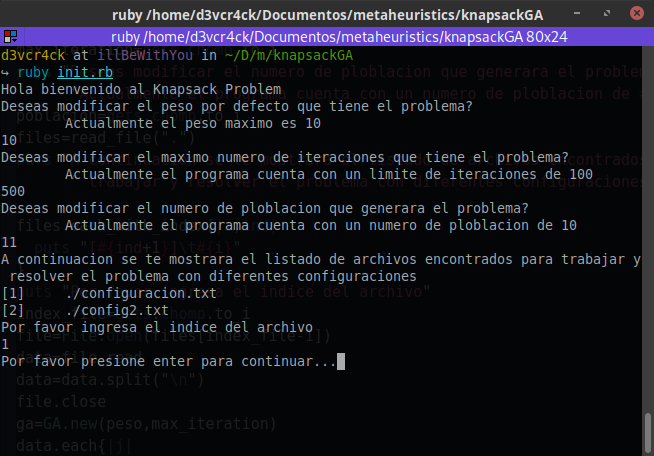
\includegraphics[scale=0.5]{imgs/ventana-knapsack.png}
  \\\textit{Figura 1: Ventana de la interfaz de datos solicitados para la solución}
  \\
  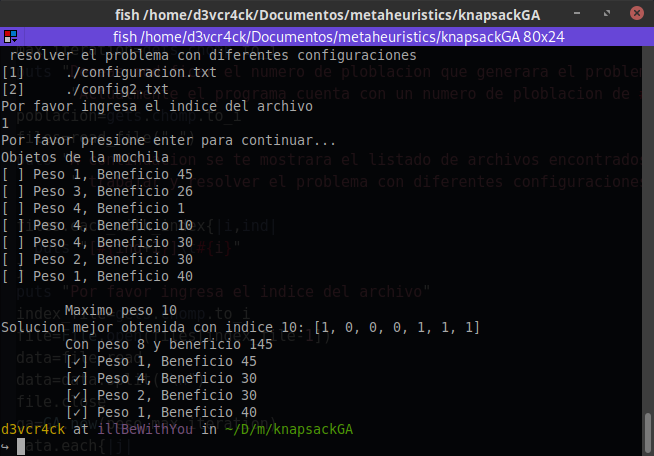
\includegraphics[scale=0.5]{imgs/ventana-knapsack-sol.png}
  \\\textit{Figura 2: Ventana de la interfaz con la solución dada por el programa}
\end{center}

\subsection{Travel Salesman Problem (TSP)}
\begin{center}
  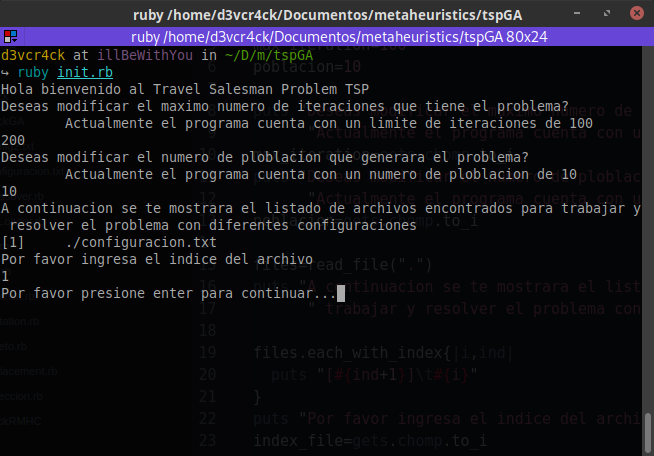
\includegraphics[scale=0.5]{imgs/ventana-tsp.png}
  \\\textit{Figura 3: Ventana de la interfaz de datos solicitados para la solución}
  \\
  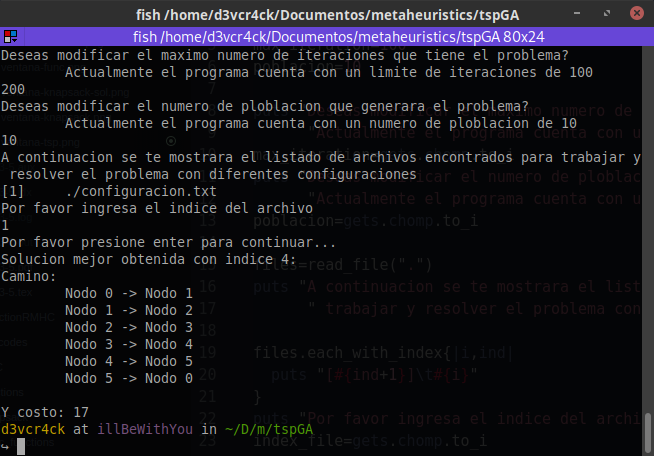
\includegraphics[scale=0.5]{imgs/ventana-tsp-sol.png}
  \\\textit{Figura 4: Ventana de la interfaz con la solución dada por el programa}
\end{center}
\subsection{Función de Minimización en D dimensiones}
\begin{center}
  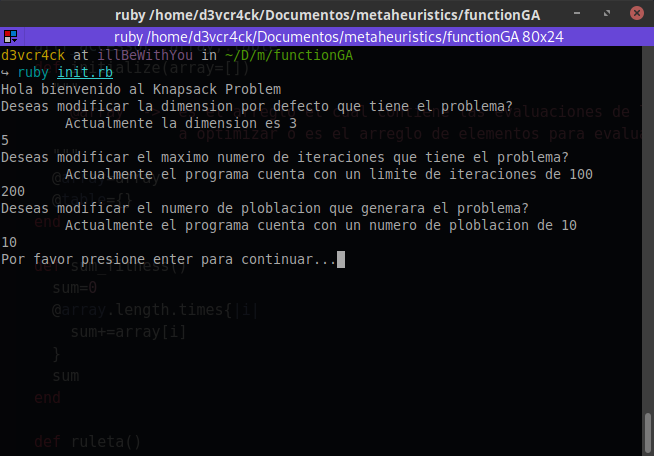
\includegraphics[scale=0.5]{imgs/ventana-func.png}
  \\\textit{Figura 5: Ventana de la interfaz de datos solicitados para la solución}
  \\
  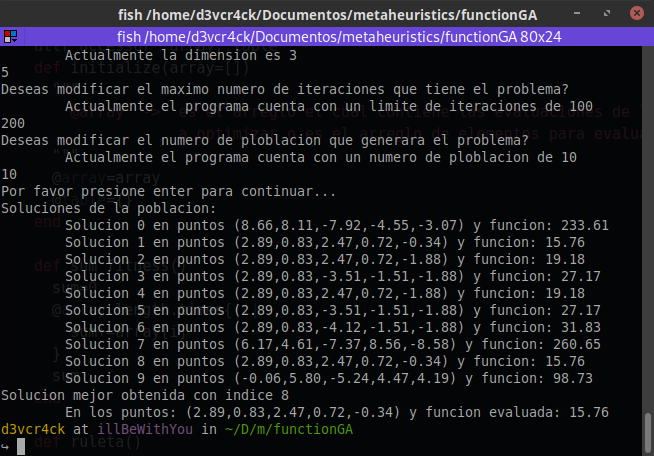
\includegraphics[scale=0.5]{imgs/ventana-func-sol.png}
  \\\textit{Figura 6: Ventana de la interfaz con la solución dada por el programa}
\end{center}



\end{document}
